% Created by tikzDevice version 0.12.3 on 2020-02-03 16:07:12
% !TEX encoding = UTF-8 Unicode
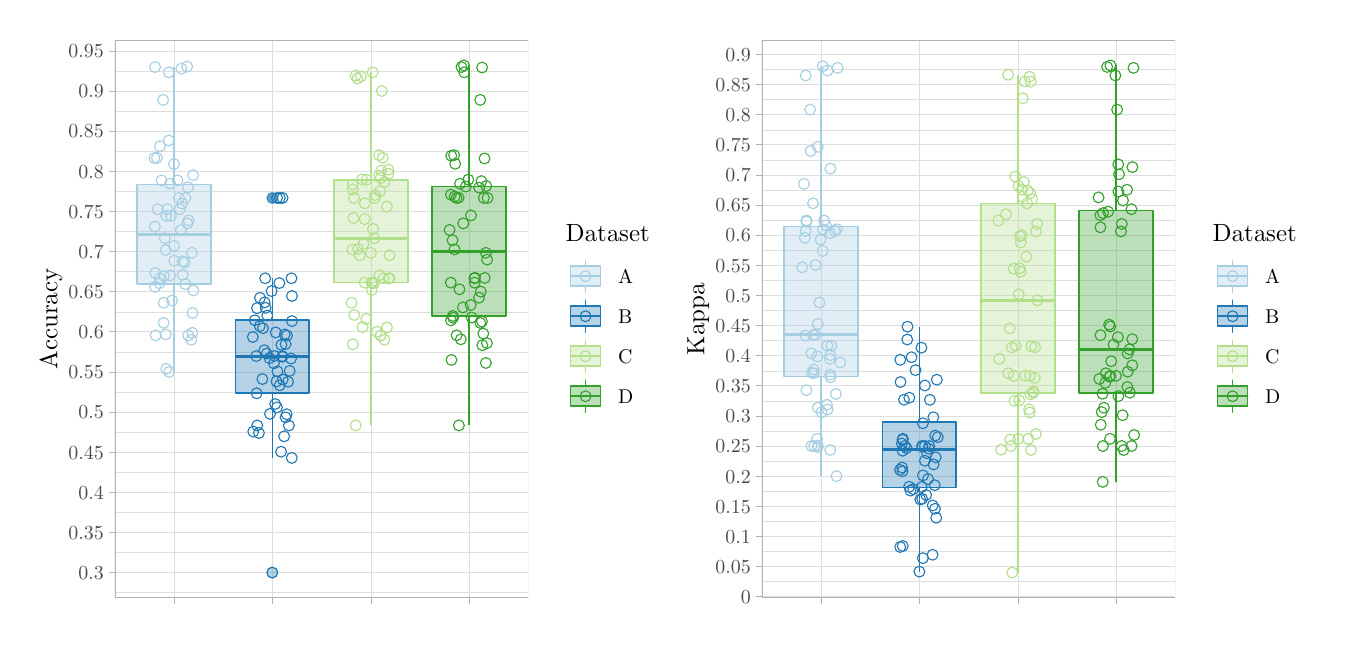
\begin{tikzpicture}[x=1pt,y=1pt]
\definecolor{fillColor}{RGB}{255,255,255}
\path[use as bounding box,fill=fillColor,fill opacity=0.00] (0,0) rectangle (467.59,216.81);
\begin{scope}
\path[clip] (  0.00,  0.00) rectangle (233.79,216.81);
\definecolor{drawColor}{RGB}{255,255,255}
\definecolor{fillColor}{RGB}{255,255,255}

\path[draw=drawColor,line width= 0.5pt,line join=round,line cap=round,fill=fillColor] (  0.00,  0.00) rectangle (233.79,216.81);
\end{scope}
\begin{scope}
\path[clip] ( 31.54, 10.75) rectangle (180.88,212.31);
\definecolor{fillColor}{RGB}{255,255,255}

\path[fill=fillColor] ( 31.54, 10.75) rectangle (180.88,212.31);
\definecolor{drawColor}{gray}{0.87}

\path[draw=drawColor,line width= 0.1pt,line join=round] ( 31.54, 12.66) --
	(180.88, 12.66);

\path[draw=drawColor,line width= 0.1pt,line join=round] ( 31.54, 27.16) --
	(180.88, 27.16);

\path[draw=drawColor,line width= 0.1pt,line join=round] ( 31.54, 41.67) --
	(180.88, 41.67);

\path[draw=drawColor,line width= 0.1pt,line join=round] ( 31.54, 56.17) --
	(180.88, 56.17);

\path[draw=drawColor,line width= 0.1pt,line join=round] ( 31.54, 70.67) --
	(180.88, 70.67);

\path[draw=drawColor,line width= 0.1pt,line join=round] ( 31.54, 85.17) --
	(180.88, 85.17);

\path[draw=drawColor,line width= 0.1pt,line join=round] ( 31.54, 99.67) --
	(180.88, 99.67);

\path[draw=drawColor,line width= 0.1pt,line join=round] ( 31.54,114.18) --
	(180.88,114.18);

\path[draw=drawColor,line width= 0.1pt,line join=round] ( 31.54,128.68) --
	(180.88,128.68);

\path[draw=drawColor,line width= 0.1pt,line join=round] ( 31.54,143.18) --
	(180.88,143.18);

\path[draw=drawColor,line width= 0.1pt,line join=round] ( 31.54,157.68) --
	(180.88,157.68);

\path[draw=drawColor,line width= 0.1pt,line join=round] ( 31.54,172.19) --
	(180.88,172.19);

\path[draw=drawColor,line width= 0.1pt,line join=round] ( 31.54,186.69) --
	(180.88,186.69);

\path[draw=drawColor,line width= 0.1pt,line join=round] ( 31.54,201.19) --
	(180.88,201.19);

\path[draw=drawColor,line width= 0.2pt,line join=round] ( 31.54, 19.91) --
	(180.88, 19.91);

\path[draw=drawColor,line width= 0.2pt,line join=round] ( 31.54, 34.41) --
	(180.88, 34.41);

\path[draw=drawColor,line width= 0.2pt,line join=round] ( 31.54, 48.92) --
	(180.88, 48.92);

\path[draw=drawColor,line width= 0.2pt,line join=round] ( 31.54, 63.42) --
	(180.88, 63.42);

\path[draw=drawColor,line width= 0.2pt,line join=round] ( 31.54, 77.92) --
	(180.88, 77.92);

\path[draw=drawColor,line width= 0.2pt,line join=round] ( 31.54, 92.42) --
	(180.88, 92.42);

\path[draw=drawColor,line width= 0.2pt,line join=round] ( 31.54,106.93) --
	(180.88,106.93);

\path[draw=drawColor,line width= 0.2pt,line join=round] ( 31.54,121.43) --
	(180.88,121.43);

\path[draw=drawColor,line width= 0.2pt,line join=round] ( 31.54,135.93) --
	(180.88,135.93);

\path[draw=drawColor,line width= 0.2pt,line join=round] ( 31.54,150.43) --
	(180.88,150.43);

\path[draw=drawColor,line width= 0.2pt,line join=round] ( 31.54,164.94) --
	(180.88,164.94);

\path[draw=drawColor,line width= 0.2pt,line join=round] ( 31.54,179.44) --
	(180.88,179.44);

\path[draw=drawColor,line width= 0.2pt,line join=round] ( 31.54,193.94) --
	(180.88,193.94);

\path[draw=drawColor,line width= 0.2pt,line join=round] ( 31.54,208.44) --
	(180.88,208.44);

\path[draw=drawColor,line width= 0.2pt,line join=round] ( 52.88, 10.75) --
	( 52.88,212.31);

\path[draw=drawColor,line width= 0.2pt,line join=round] ( 88.43, 10.75) --
	( 88.43,212.31);

\path[draw=drawColor,line width= 0.2pt,line join=round] (123.99, 10.75) --
	(123.99,212.31);

\path[draw=drawColor,line width= 0.2pt,line join=round] (159.54, 10.75) --
	(159.54,212.31);
\definecolor{drawColor}{RGB}{166,206,227}

\path[draw=drawColor,line width= 0.6pt,line join=round] ( 52.88,160.14) -- ( 52.88,202.75);

\path[draw=drawColor,line width= 0.6pt,line join=round] ( 52.88,124.23) -- ( 52.88, 92.42);
\definecolor{fillColor}{RGB}{166,206,227}

\path[draw=drawColor,line width= 0.6pt,line join=round,line cap=round,fill=fillColor,fill opacity=0.33] ( 39.54,160.14) --
	( 39.54,124.23) --
	( 66.21,124.23) --
	( 66.21,160.14) --
	( 39.54,160.14) --
	cycle;

\path[draw=drawColor,line width= 1.1pt,line join=round] ( 39.54,142.23) -- ( 66.21,142.23);
\definecolor{drawColor}{RGB}{31,120,180}
\definecolor{fillColor}{RGB}{31,120,180}

\path[draw=drawColor,draw opacity=0.33,line width= 0.4pt,line join=round,line cap=round,fill=fillColor,fill opacity=0.33] ( 88.43,155.27) circle (  1.96);

\path[draw=drawColor,draw opacity=0.33,line width= 0.4pt,line join=round,line cap=round,fill=fillColor,fill opacity=0.33] ( 88.43, 19.91) circle (  1.96);

\path[draw=drawColor,draw opacity=0.33,line width= 0.4pt,line join=round,line cap=round,fill=fillColor,fill opacity=0.33] ( 88.43,155.27) circle (  1.96);

\path[draw=drawColor,draw opacity=0.33,line width= 0.4pt,line join=round,line cap=round,fill=fillColor,fill opacity=0.33] ( 88.43,155.27) circle (  1.96);
\definecolor{drawColor}{RGB}{31,120,180}

\path[draw=drawColor,line width= 0.6pt,line join=round] ( 88.43,111.10) -- ( 88.43,126.26);

\path[draw=drawColor,line width= 0.6pt,line join=round] ( 88.43, 84.69) -- ( 88.43, 61.35);

\path[draw=drawColor,line width= 0.6pt,line join=round,line cap=round,fill=fillColor,fill opacity=0.33] ( 75.10,111.10) --
	( 75.10, 84.69) --
	(101.77, 84.69) --
	(101.77,111.10) --
	( 75.10,111.10) --
	cycle;

\path[draw=drawColor,line width= 1.1pt,line join=round] ( 75.10, 98.14) -- (101.77, 98.14);
\definecolor{drawColor}{RGB}{178,223,138}

\path[draw=drawColor,line width= 0.6pt,line join=round] (123.99,161.82) -- (123.99,200.67);

\path[draw=drawColor,line width= 0.6pt,line join=round] (123.99,124.68) -- (123.99, 73.09);
\definecolor{fillColor}{RGB}{178,223,138}

\path[draw=drawColor,line width= 0.6pt,line join=round,line cap=round,fill=fillColor,fill opacity=0.33] (110.65,161.82) --
	(110.65,124.68) --
	(137.32,124.68) --
	(137.32,161.82) --
	(110.65,161.82) --
	cycle;

\path[draw=drawColor,line width= 1.1pt,line join=round] (110.65,140.76) -- (137.32,140.76);
\definecolor{drawColor}{RGB}{51,160,44}

\path[draw=drawColor,line width= 0.6pt,line join=round] (159.54,159.45) -- (159.54,203.15);

\path[draw=drawColor,line width= 0.6pt,line join=round] (159.54,112.51) -- (159.54, 73.09);
\definecolor{fillColor}{RGB}{51,160,44}

\path[draw=drawColor,line width= 0.6pt,line join=round,line cap=round,fill=fillColor,fill opacity=0.33] (146.21,159.45) --
	(146.21,112.51) --
	(172.88,112.51) --
	(172.88,159.45) --
	(146.21,159.45) --
	cycle;

\path[draw=drawColor,line width= 1.1pt,line join=round] (146.21,136.06) -- (172.88,136.06);
\definecolor{drawColor}{RGB}{166,206,227}

\path[draw=drawColor,line width= 0.4pt,line join=round,line cap=round] ( 51.49,160.48) circle (  1.96);

\path[draw=drawColor,line width= 0.4pt,line join=round,line cap=round] ( 45.80,169.71) circle (  1.96);

\path[draw=drawColor,line width= 0.4pt,line join=round,line cap=round] ( 59.13,104.03) circle (  1.96);

\path[draw=drawColor,line width= 0.4pt,line join=round,line cap=round] ( 51.76,148.81) circle (  1.96);

\path[draw=drawColor,line width= 0.4pt,line join=round,line cap=round] ( 56.72,132.02) circle (  1.96);

\path[draw=drawColor,line width= 0.4pt,line join=round,line cap=round] ( 58.11,147.22) circle (  1.96);

\path[draw=drawColor,line width= 0.4pt,line join=round,line cap=round] ( 48.96,190.72) circle (  1.96);

\path[draw=drawColor,line width= 0.4pt,line join=round,line cap=round] ( 56.00,132.36) circle (  1.96);

\path[draw=drawColor,line width= 0.4pt,line join=round,line cap=round] ( 59.46,106.53) circle (  1.96);

\path[draw=drawColor,line width= 0.4pt,line join=round,line cap=round] ( 55.38,143.70) circle (  1.96);

\path[draw=drawColor,line width= 0.4pt,line join=round,line cap=round] ( 49.54,140.76) circle (  1.96);

\path[draw=drawColor,line width= 0.4pt,line join=round,line cap=round] ( 57.90,159.11) circle (  1.96);

\path[draw=drawColor,line width= 0.4pt,line join=round,line cap=round] ( 47.78,173.99) circle (  1.96);

\path[draw=drawColor,line width= 0.4pt,line join=round,line cap=round] ( 46.25,105.64) circle (  1.96);

\path[draw=drawColor,line width= 0.4pt,line join=round,line cap=round] ( 46.98,151.22) circle (  1.96);

\path[draw=drawColor,line width= 0.4pt,line join=round,line cap=round] ( 51.49,127.32) circle (  1.96);

\path[draw=drawColor,line width= 0.4pt,line join=round,line cap=round] ( 49.90,136.49) circle (  1.96);

\path[draw=drawColor,line width= 0.4pt,line join=round,line cap=round] ( 55.55,202.00) circle (  1.96);

\path[draw=drawColor,line width= 0.4pt,line join=round,line cap=round] ( 46.06,123.16) circle (  1.96);

\path[draw=drawColor,line width= 0.4pt,line join=round,line cap=round] ( 58.00,105.56) circle (  1.96);

\path[draw=drawColor,line width= 0.4pt,line join=round,line cap=round] ( 57.75,146.08) circle (  1.96);

\path[draw=drawColor,line width= 0.4pt,line join=round,line cap=round] ( 47.67,126.26) circle (  1.96);

\path[draw=drawColor,line width= 0.4pt,line join=round,line cap=round] ( 48.38,161.62) circle (  1.96);

\path[draw=drawColor,line width= 0.4pt,line join=round,line cap=round] ( 51.02,176.04) circle (  1.96);

\path[draw=drawColor,line width= 0.4pt,line join=round,line cap=round] ( 52.17,118.21) circle (  1.96);

\path[draw=drawColor,line width= 0.4pt,line join=round,line cap=round] ( 50.50,151.22) circle (  1.96);

\path[draw=drawColor,line width= 0.4pt,line join=round,line cap=round] ( 55.99,127.49) circle (  1.96);

\path[draw=drawColor,line width= 0.4pt,line join=round,line cap=round] ( 52.85,137.94) circle (  1.96);

\path[draw=drawColor,line width= 0.4pt,line join=round,line cap=round] ( 51.01,200.67) circle (  1.96);

\path[draw=drawColor,line width= 0.4pt,line join=round,line cap=round] ( 46.12,128.20) circle (  1.96);

\path[draw=drawColor,line width= 0.4pt,line join=round,line cap=round] ( 49.89,106.00) circle (  1.96);

\path[draw=drawColor,line width= 0.4pt,line join=round,line cap=round] ( 59.35,135.45) circle (  1.96);

\path[draw=drawColor,line width= 0.4pt,line join=round,line cap=round] ( 56.98,155.27) circle (  1.96);

\path[draw=drawColor,line width= 0.4pt,line join=round,line cap=round] ( 54.14,161.62) circle (  1.96);

\path[draw=drawColor,line width= 0.4pt,line join=round,line cap=round] ( 59.79,163.53) circle (  1.96);

\path[draw=drawColor,line width= 0.4pt,line join=round,line cap=round] ( 49.13,110.15) circle (  1.96);

\path[draw=drawColor,line width= 0.4pt,line join=round,line cap=round] ( 54.98,151.22) circle (  1.96);

\path[draw=drawColor,line width= 0.4pt,line join=round,line cap=round] ( 52.94,132.59) circle (  1.96);

\path[draw=drawColor,line width= 0.4pt,line join=round,line cap=round] ( 49.25,127.07) circle (  1.96);

\path[draw=drawColor,line width= 0.4pt,line join=round,line cap=round] ( 57.63,202.75) circle (  1.96);

\path[draw=drawColor,line width= 0.4pt,line join=round,line cap=round] ( 56.93,124.15) circle (  1.96);

\path[draw=drawColor,line width= 0.4pt,line join=round,line cap=round] ( 50.07, 93.52) circle (  1.96);

\path[draw=drawColor,line width= 0.4pt,line join=round,line cap=round] ( 51.11, 92.42) circle (  1.96);

\path[draw=drawColor,line width= 0.4pt,line join=round,line cap=round] ( 46.72,169.77) circle (  1.96);

\path[draw=drawColor,line width= 0.4pt,line join=round,line cap=round] ( 52.86,167.51) circle (  1.96);

\path[draw=drawColor,line width= 0.4pt,line join=round,line cap=round] ( 55.80,153.27) circle (  1.96);

\path[draw=drawColor,line width= 0.4pt,line join=round,line cap=round] ( 49.16,117.40) circle (  1.96);

\path[draw=drawColor,line width= 0.4pt,line join=round,line cap=round] ( 50.07,148.81) circle (  1.96);

\path[draw=drawColor,line width= 0.4pt,line join=round,line cap=round] ( 47.61,124.46) circle (  1.96);

\path[draw=drawColor,line width= 0.4pt,line join=round,line cap=round] ( 45.97,144.91) circle (  1.96);

\path[draw=drawColor,line width= 0.4pt,line join=round,line cap=round] ( 46.04,202.57) circle (  1.96);

\path[draw=drawColor,line width= 0.4pt,line join=round,line cap=round] ( 59.88,121.87) circle (  1.96);

\path[draw=drawColor,line width= 0.4pt,line join=round,line cap=round] ( 59.57,113.74) circle (  1.96);

\path[draw=drawColor,line width= 0.4pt,line join=round,line cap=round] ( 54.70,155.27) circle (  1.96);
\definecolor{drawColor}{RGB}{31,120,180}

\path[draw=drawColor,line width= 0.4pt,line join=round,line cap=round] ( 82.75, 84.69) circle (  1.96);

\path[draw=drawColor,line width= 0.4pt,line join=round,line cap=round] ( 82.87,115.45) circle (  1.96);

\path[draw=drawColor,line width= 0.4pt,line join=round,line cap=round] ( 89.89, 89.00) circle (  1.96);

\path[draw=drawColor,line width= 0.4pt,line join=round,line cap=round] ( 90.95,124.53) circle (  1.96);

\path[draw=drawColor,line width= 0.4pt,line join=round,line cap=round] ( 81.36,105.03) circle (  1.96);

\path[draw=drawColor,line width= 0.4pt,line join=round,line cap=round] ( 94.68, 92.78) circle (  1.96);

\path[draw=drawColor,line width= 0.4pt,line join=round,line cap=round] ( 93.19, 76.02) circle (  1.96);

\path[draw=drawColor,line width= 0.4pt,line join=round,line cap=round] ( 83.95,119.18) circle (  1.96);

\path[draw=drawColor,line width= 0.4pt,line join=round,line cap=round] ( 93.70,105.56) circle (  1.96);

\path[draw=drawColor,line width= 0.4pt,line join=round,line cap=round] ( 94.09, 88.88) circle (  1.96);

\path[draw=drawColor,line width= 0.4pt,line join=round,line cap=round] ( 95.32,126.26) circle (  1.96);

\path[draw=drawColor,line width= 0.4pt,line join=round,line cap=round] ( 89.44, 80.82) circle (  1.96);

\path[draw=drawColor,line width= 0.4pt,line join=round,line cap=round] ( 82.08,111.10) circle (  1.96);

\path[draw=drawColor,line width= 0.4pt,line join=round,line cap=round] ( 82.94, 73.07) circle (  1.96);

\path[draw=drawColor,line width= 0.4pt,line join=round,line cap=round] ( 85.99,115.57) circle (  1.96);

\path[draw=drawColor,line width= 0.4pt,line join=round,line cap=round] ( 92.87,105.96) circle (  1.96);

\path[draw=drawColor,line width= 0.4pt,line join=round,line cap=round] ( 85.50,100.25) circle (  1.96);

\path[draw=drawColor,line width= 0.4pt,line join=round,line cap=round] ( 92.16, 89.68) circle (  1.96);

\path[draw=drawColor,line width= 0.4pt,line join=round,line cap=round] ( 95.16, 97.24) circle (  1.96);

\path[draw=drawColor,line width= 0.4pt,line join=round,line cap=round] ( 89.19, 98.18) circle (  1.96);

\path[draw=drawColor,line width= 0.4pt,line join=round,line cap=round] ( 90.28, 92.60) circle (  1.96);

\path[draw=drawColor,line width= 0.4pt,line join=round,line cap=round] ( 85.83,126.26) circle (  1.96);

\path[draw=drawColor,line width= 0.4pt,line join=round,line cap=round] ( 91.57, 63.58) circle (  1.96);

\path[draw=drawColor,line width= 0.4pt,line join=round,line cap=round] ( 95.50,119.86) circle (  1.96);

\path[draw=drawColor,line width= 0.4pt,line join=round,line cap=round] ( 87.55, 77.25) circle (  1.96);

\path[draw=drawColor,line width= 0.4pt,line join=round,line cap=round] ( 83.87,108.98) circle (  1.96);

\path[draw=drawColor,line width= 0.4pt,line join=round,line cap=round] ( 91.07, 87.59) circle (  1.96);

\path[draw=drawColor,line width= 0.4pt,line join=round,line cap=round] ( 92.01, 98.14) circle (  1.96);

\path[draw=drawColor,line width= 0.4pt,line join=round,line cap=round] ( 90.08, 79.61) circle (  1.96);

\path[draw=drawColor,line width= 0.4pt,line join=round,line cap=round] ( 84.82, 89.83) circle (  1.96);

\path[draw=drawColor,line width= 0.4pt,line join=round,line cap=round] ( 88.99, 95.50) circle (  1.96);

\path[draw=drawColor,line width= 0.4pt,line join=round,line cap=round] ( 86.37, 99.04) circle (  1.96);

\path[draw=drawColor,line width= 0.4pt,line join=round,line cap=round] ( 91.11,155.27) circle (  1.96);

\path[draw=drawColor,line width= 0.4pt,line join=round,line cap=round] ( 92.68, 69.14) circle (  1.96);

\path[draw=drawColor,line width= 0.4pt,line join=round,line cap=round] ( 85.03,108.20) circle (  1.96);

\path[draw=drawColor,line width= 0.4pt,line join=round,line cap=round] ( 94.38, 73.06) circle (  1.96);

\path[draw=drawColor,line width= 0.4pt,line join=round,line cap=round] ( 95.50,110.79) circle (  1.96);

\path[draw=drawColor,line width= 0.4pt,line join=round,line cap=round] ( 88.36, 19.91) circle (  1.96);

\path[draw=drawColor,line width= 0.4pt,line join=round,line cap=round] ( 82.61, 98.14) circle (  1.96);

\path[draw=drawColor,line width= 0.4pt,line join=round,line cap=round] ( 93.59, 77.12) circle (  1.96);

\path[draw=drawColor,line width= 0.4pt,line join=round,line cap=round] ( 88.16,121.63) circle (  1.96);

\path[draw=drawColor,line width= 0.4pt,line join=round,line cap=round] ( 92.00, 97.87) circle (  1.96);

\path[draw=drawColor,line width= 0.4pt,line join=round,line cap=round] ( 93.20,102.49) circle (  1.96);

\path[draw=drawColor,line width= 0.4pt,line join=round,line cap=round] ( 90.09,155.27) circle (  1.96);

\path[draw=drawColor,line width= 0.4pt,line join=round,line cap=round] ( 83.57, 70.35) circle (  1.96);

\path[draw=drawColor,line width= 0.4pt,line join=round,line cap=round] ( 91.68,102.18) circle (  1.96);

\path[draw=drawColor,line width= 0.4pt,line join=round,line cap=round] ( 81.52, 70.86) circle (  1.96);

\path[draw=drawColor,line width= 0.4pt,line join=round,line cap=round] ( 85.63,117.56) circle (  1.96);

\path[draw=drawColor,line width= 0.4pt,line join=round,line cap=round] ( 86.58,112.77) circle (  1.96);

\path[draw=drawColor,line width= 0.4pt,line join=round,line cap=round] ( 95.44, 61.35) circle (  1.96);

\path[draw=drawColor,line width= 0.4pt,line join=round,line cap=round] ( 89.65,106.69) circle (  1.96);

\path[draw=drawColor,line width= 0.4pt,line join=round,line cap=round] ( 87.36, 97.39) circle (  1.96);

\path[draw=drawColor,line width= 0.4pt,line join=round,line cap=round] ( 92.10,155.27) circle (  1.96);
\definecolor{drawColor}{RGB}{178,223,138}

\path[draw=drawColor,line width= 0.4pt,line join=round,line cap=round] (127.00,163.38) circle (  1.96);

\path[draw=drawColor,line width= 0.4pt,line join=round,line cap=round] (130.32,165.51) circle (  1.96);

\path[draw=drawColor,line width= 0.4pt,line join=round,line cap=round] (126.13,106.93) circle (  1.96);

\path[draw=drawColor,line width= 0.4pt,line join=round,line cap=round] (122.48,161.82) circle (  1.96);

\path[draw=drawColor,line width= 0.4pt,line join=round,line cap=round] (130.44,126.17) circle (  1.96);

\path[draw=drawColor,line width= 0.4pt,line join=round,line cap=round] (124.79,144.05) circle (  1.96);

\path[draw=drawColor,line width= 0.4pt,line join=round,line cap=round] (127.96,193.94) circle (  1.96);

\path[draw=drawColor,line width= 0.4pt,line join=round,line cap=round] (130.77,134.59) circle (  1.96);

\path[draw=drawColor,line width= 0.4pt,line join=round,line cap=round] (121.01,108.64) circle (  1.96);

\path[draw=drawColor,line width= 0.4pt,line join=round,line cap=round] (129.82,152.16) circle (  1.96);

\path[draw=drawColor,line width= 0.4pt,line join=round,line cap=round] (128.62,126.26) circle (  1.96);

\path[draw=drawColor,line width= 0.4pt,line join=round,line cap=round] (120.89,162.01) circle (  1.96);

\path[draw=drawColor,line width= 0.4pt,line join=round,line cap=round] (117.45,160.13) circle (  1.96);

\path[draw=drawColor,line width= 0.4pt,line join=round,line cap=round] (127.63,105.64) circle (  1.96);

\path[draw=drawColor,line width= 0.4pt,line join=round,line cap=round] (127.60,162.52) circle (  1.96);

\path[draw=drawColor,line width= 0.4pt,line join=round,line cap=round] (121.73,124.68) circle (  1.96);

\path[draw=drawColor,line width= 0.4pt,line join=round,line cap=round] (121.76,147.61) circle (  1.96);

\path[draw=drawColor,line width= 0.4pt,line join=round,line cap=round] (120.43,199.18) circle (  1.96);

\path[draw=drawColor,line width= 0.4pt,line join=round,line cap=round] (125.22,124.50) circle (  1.96);

\path[draw=drawColor,line width= 0.4pt,line join=round,line cap=round] (127.48,105.52) circle (  1.96);

\path[draw=drawColor,line width= 0.4pt,line join=round,line cap=round] (121.80,153.33) circle (  1.96);

\path[draw=drawColor,line width= 0.4pt,line join=round,line cap=round] (130.78,126.26) circle (  1.96);

\path[draw=drawColor,line width= 0.4pt,line join=round,line cap=round] (117.43,158.40) circle (  1.96);

\path[draw=drawColor,line width= 0.4pt,line join=round,line cap=round] (128.91,161.05) circle (  1.96);

\path[draw=drawColor,line width= 0.4pt,line join=round,line cap=round] (117.49,102.41) circle (  1.96);

\path[draw=drawColor,line width= 0.4pt,line join=round,line cap=round] (130.37,164.07) circle (  1.96);

\path[draw=drawColor,line width= 0.4pt,line join=round,line cap=round] (124.23,124.68) circle (  1.96);

\path[draw=drawColor,line width= 0.4pt,line join=round,line cap=round] (125.21,140.76) circle (  1.96);

\path[draw=drawColor,line width= 0.4pt,line join=round,line cap=round] (124.66,200.67) circle (  1.96);

\path[draw=drawColor,line width= 0.4pt,line join=round,line cap=round] (127.09,127.35) circle (  1.96);

\path[draw=drawColor,line width= 0.4pt,line join=round,line cap=round] (118.01,112.99) circle (  1.96);

\path[draw=drawColor,line width= 0.4pt,line join=round,line cap=round] (124.03,135.45) circle (  1.96);

\path[draw=drawColor,line width= 0.4pt,line join=round,line cap=round] (125.58,155.27) circle (  1.96);

\path[draw=drawColor,line width= 0.4pt,line join=round,line cap=round] (125.50,156.35) circle (  1.96);

\path[draw=drawColor,line width= 0.4pt,line join=round,line cap=round] (127.33,157.73) circle (  1.96);

\path[draw=drawColor,line width= 0.4pt,line join=round,line cap=round] (128.93,104.03) circle (  1.96);

\path[draw=drawColor,line width= 0.4pt,line join=round,line cap=round] (127.75,165.20) circle (  1.96);

\path[draw=drawColor,line width= 0.4pt,line join=round,line cap=round] (124.63,124.68) circle (  1.96);

\path[draw=drawColor,line width= 0.4pt,line join=round,line cap=round] (117.73,148.02) circle (  1.96);

\path[draw=drawColor,line width= 0.4pt,line join=round,line cap=round] (118.49,199.52) circle (  1.96);

\path[draw=drawColor,line width= 0.4pt,line join=round,line cap=round] (119.43,136.84) circle (  1.96);

\path[draw=drawColor,line width= 0.4pt,line join=round,line cap=round] (122.34,111.54) circle (  1.96);

\path[draw=drawColor,line width= 0.4pt,line join=round,line cap=round] (118.55, 73.09) circle (  1.96);

\path[draw=drawColor,line width= 0.4pt,line join=round,line cap=round] (128.31,169.77) circle (  1.96);

\path[draw=drawColor,line width= 0.4pt,line join=round,line cap=round] (126.95,170.74) circle (  1.96);

\path[draw=drawColor,line width= 0.4pt,line join=round,line cap=round] (117.32,136.60) circle (  1.96);

\path[draw=drawColor,line width= 0.4pt,line join=round,line cap=round] (117.06,117.40) circle (  1.96);

\path[draw=drawColor,line width= 0.4pt,line join=round,line cap=round] (124.35,122.04) circle (  1.96);

\path[draw=drawColor,line width= 0.4pt,line join=round,line cap=round] (121.36,138.69) circle (  1.96);

\path[draw=drawColor,line width= 0.4pt,line join=round,line cap=round] (119.15,198.43) circle (  1.96);

\path[draw=drawColor,line width= 0.4pt,line join=round,line cap=round] (120.03,134.58) circle (  1.96);

\path[draw=drawColor,line width= 0.4pt,line join=round,line cap=round] (129.83,108.46) circle (  1.96);

\path[draw=drawColor,line width= 0.4pt,line join=round,line cap=round] (117.94,155.27) circle (  1.96);
\definecolor{drawColor}{RGB}{51,160,44}

\path[draw=drawColor,line width= 0.4pt,line join=round,line cap=round] (156.22,160.42) circle (  1.96);

\path[draw=drawColor,line width= 0.4pt,line join=round,line cap=round] (159.22,161.90) circle (  1.96);

\path[draw=drawColor,line width= 0.4pt,line join=round,line cap=round] (160.43,112.08) circle (  1.96);

\path[draw=drawColor,line width= 0.4pt,line join=round,line cap=round] (158.32,159.40) circle (  1.96);

\path[draw=drawColor,line width= 0.4pt,line join=round,line cap=round] (161.60,126.44) circle (  1.96);

\path[draw=drawColor,line width= 0.4pt,line join=round,line cap=round] (165.95,102.82) circle (  1.96);

\path[draw=drawColor,line width= 0.4pt,line join=round,line cap=round] (163.53,190.72) circle (  1.96);

\path[draw=drawColor,line width= 0.4pt,line join=round,line cap=round] (153.52,139.99) circle (  1.96);

\path[draw=drawColor,line width= 0.4pt,line join=round,line cap=round] (164.63,106.27) circle (  1.96);

\path[draw=drawColor,line width= 0.4pt,line join=round,line cap=round] (152.45,143.70) circle (  1.96);

\path[draw=drawColor,line width= 0.4pt,line join=round,line cap=round] (160.06,116.59) circle (  1.96);

\path[draw=drawColor,line width= 0.4pt,line join=round,line cap=round] (152.95,156.47) circle (  1.96);

\path[draw=drawColor,line width= 0.4pt,line join=round,line cap=round] (165.69,159.59) circle (  1.96);

\path[draw=drawColor,line width= 0.4pt,line join=round,line cap=round] (155.01,105.64) circle (  1.96);

\path[draw=drawColor,line width= 0.4pt,line join=round,line cap=round] (153.06,170.52) circle (  1.96);

\path[draw=drawColor,line width= 0.4pt,line join=round,line cap=round] (152.88,124.68) circle (  1.96);

\path[draw=drawColor,line width= 0.4pt,line join=round,line cap=round] (153.73,112.00) circle (  1.96);

\path[draw=drawColor,line width= 0.4pt,line join=round,line cap=round] (164.21,202.40) circle (  1.96);

\path[draw=drawColor,line width= 0.4pt,line join=round,line cap=round] (165.14,126.38) circle (  1.96);

\path[draw=drawColor,line width= 0.4pt,line join=round,line cap=round] (164.16,110.62) circle (  1.96);

\path[draw=drawColor,line width= 0.4pt,line join=round,line cap=round] (157.42,146.08) circle (  1.96);

\path[draw=drawColor,line width= 0.4pt,line join=round,line cap=round] (161.44,126.26) circle (  1.96);

\path[draw=drawColor,line width= 0.4pt,line join=round,line cap=round] (163.13,158.99) circle (  1.96);

\path[draw=drawColor,line width= 0.4pt,line join=round,line cap=round] (155.71,155.37) circle (  1.96);

\path[draw=drawColor,line width= 0.4pt,line join=round,line cap=round] (165.56, 95.65) circle (  1.96);

\path[draw=drawColor,line width= 0.4pt,line join=round,line cap=round] (161.50,124.68) circle (  1.96);

\path[draw=drawColor,line width= 0.4pt,line join=round,line cap=round] (152.94,111.03) circle (  1.96);

\path[draw=drawColor,line width= 0.4pt,line join=round,line cap=round] (157.75,200.67) circle (  1.96);

\path[draw=drawColor,line width= 0.4pt,line join=round,line cap=round] (166.01,132.99) circle (  1.96);

\path[draw=drawColor,line width= 0.4pt,line join=round,line cap=round] (157.28,115.72) circle (  1.96);

\path[draw=drawColor,line width= 0.4pt,line join=round,line cap=round] (165.58,135.45) circle (  1.96);

\path[draw=drawColor,line width= 0.4pt,line join=round,line cap=round] (154.95,155.27) circle (  1.96);

\path[draw=drawColor,line width= 0.4pt,line join=round,line cap=round] (163.96,161.36) circle (  1.96);

\path[draw=drawColor,line width= 0.4pt,line join=round,line cap=round] (160.19,148.97) circle (  1.96);

\path[draw=drawColor,line width= 0.4pt,line join=round,line cap=round] (153.64,112.65) circle (  1.96);

\path[draw=drawColor,line width= 0.4pt,line join=round,line cap=round] (165.08,169.55) circle (  1.96);

\path[draw=drawColor,line width= 0.4pt,line join=round,line cap=round] (156.04,122.26) circle (  1.96);

\path[draw=drawColor,line width= 0.4pt,line join=round,line cap=round] (164.29,102.09) circle (  1.96);

\path[draw=drawColor,line width= 0.4pt,line join=round,line cap=round] (157.63,203.15) circle (  1.96);

\path[draw=drawColor,line width= 0.4pt,line join=round,line cap=round] (154.24,136.68) circle (  1.96);

\path[draw=drawColor,line width= 0.4pt,line join=round,line cap=round] (163.54,110.13) circle (  1.96);

\path[draw=drawColor,line width= 0.4pt,line join=round,line cap=round] (155.82, 73.09) circle (  1.96);

\path[draw=drawColor,line width= 0.4pt,line join=round,line cap=round] (166.18,155.27) circle (  1.96);

\path[draw=drawColor,line width= 0.4pt,line join=round,line cap=round] (154.08,170.74) circle (  1.96);

\path[draw=drawColor,line width= 0.4pt,line join=round,line cap=round] (154.29,155.79) circle (  1.96);

\path[draw=drawColor,line width= 0.4pt,line join=round,line cap=round] (156.51,104.19) circle (  1.96);

\path[draw=drawColor,line width= 0.4pt,line join=round,line cap=round] (154.48,167.62) circle (  1.96);

\path[draw=drawColor,line width= 0.4pt,line join=round,line cap=round] (163.72,121.43) circle (  1.96);

\path[draw=drawColor,line width= 0.4pt,line join=round,line cap=round] (153.13, 96.74) circle (  1.96);

\path[draw=drawColor,line width= 0.4pt,line join=round,line cap=round] (156.74,202.57) circle (  1.96);

\path[draw=drawColor,line width= 0.4pt,line join=round,line cap=round] (163.08,119.23) circle (  1.96);

\path[draw=drawColor,line width= 0.4pt,line join=round,line cap=round] (164.85,155.27) circle (  1.96);
\definecolor{drawColor}{gray}{0.70}

\path[draw=drawColor,line width= 0.5pt,line join=round,line cap=round] ( 31.54, 10.75) rectangle (180.88,212.31);
\end{scope}
\begin{scope}
\path[clip] (  0.00,  0.00) rectangle (467.59,216.81);
\definecolor{drawColor}{gray}{0.30}

\node[text=drawColor,anchor=base east,inner sep=0pt, outer sep=0pt, scale=  0.72] at ( 27.49, 17.43) {0.3};

\node[text=drawColor,anchor=base east,inner sep=0pt, outer sep=0pt, scale=  0.72] at ( 27.49, 31.93) {0.35};

\node[text=drawColor,anchor=base east,inner sep=0pt, outer sep=0pt, scale=  0.72] at ( 27.49, 46.44) {0.4};

\node[text=drawColor,anchor=base east,inner sep=0pt, outer sep=0pt, scale=  0.72] at ( 27.49, 60.94) {0.45};

\node[text=drawColor,anchor=base east,inner sep=0pt, outer sep=0pt, scale=  0.72] at ( 27.49, 75.44) {0.5};

\node[text=drawColor,anchor=base east,inner sep=0pt, outer sep=0pt, scale=  0.72] at ( 27.49, 89.94) {0.55};

\node[text=drawColor,anchor=base east,inner sep=0pt, outer sep=0pt, scale=  0.72] at ( 27.49,104.45) {0.6};

\node[text=drawColor,anchor=base east,inner sep=0pt, outer sep=0pt, scale=  0.72] at ( 27.49,118.95) {0.65};

\node[text=drawColor,anchor=base east,inner sep=0pt, outer sep=0pt, scale=  0.72] at ( 27.49,133.45) {0.7};

\node[text=drawColor,anchor=base east,inner sep=0pt, outer sep=0pt, scale=  0.72] at ( 27.49,147.95) {0.75};

\node[text=drawColor,anchor=base east,inner sep=0pt, outer sep=0pt, scale=  0.72] at ( 27.49,162.46) {0.8};

\node[text=drawColor,anchor=base east,inner sep=0pt, outer sep=0pt, scale=  0.72] at ( 27.49,176.96) {0.85};

\node[text=drawColor,anchor=base east,inner sep=0pt, outer sep=0pt, scale=  0.72] at ( 27.49,191.46) {0.9};

\node[text=drawColor,anchor=base east,inner sep=0pt, outer sep=0pt, scale=  0.72] at ( 27.49,205.96) {0.95};
\end{scope}
\begin{scope}
\path[clip] (  0.00,  0.00) rectangle (467.59,216.81);
\definecolor{drawColor}{gray}{0.70}

\path[draw=drawColor,line width= 0.2pt,line join=round] ( 29.29, 19.91) --
	( 31.54, 19.91);

\path[draw=drawColor,line width= 0.2pt,line join=round] ( 29.29, 34.41) --
	( 31.54, 34.41);

\path[draw=drawColor,line width= 0.2pt,line join=round] ( 29.29, 48.92) --
	( 31.54, 48.92);

\path[draw=drawColor,line width= 0.2pt,line join=round] ( 29.29, 63.42) --
	( 31.54, 63.42);

\path[draw=drawColor,line width= 0.2pt,line join=round] ( 29.29, 77.92) --
	( 31.54, 77.92);

\path[draw=drawColor,line width= 0.2pt,line join=round] ( 29.29, 92.42) --
	( 31.54, 92.42);

\path[draw=drawColor,line width= 0.2pt,line join=round] ( 29.29,106.93) --
	( 31.54,106.93);

\path[draw=drawColor,line width= 0.2pt,line join=round] ( 29.29,121.43) --
	( 31.54,121.43);

\path[draw=drawColor,line width= 0.2pt,line join=round] ( 29.29,135.93) --
	( 31.54,135.93);

\path[draw=drawColor,line width= 0.2pt,line join=round] ( 29.29,150.43) --
	( 31.54,150.43);

\path[draw=drawColor,line width= 0.2pt,line join=round] ( 29.29,164.94) --
	( 31.54,164.94);

\path[draw=drawColor,line width= 0.2pt,line join=round] ( 29.29,179.44) --
	( 31.54,179.44);

\path[draw=drawColor,line width= 0.2pt,line join=round] ( 29.29,193.94) --
	( 31.54,193.94);

\path[draw=drawColor,line width= 0.2pt,line join=round] ( 29.29,208.44) --
	( 31.54,208.44);
\end{scope}
\begin{scope}
\path[clip] (  0.00,  0.00) rectangle (467.59,216.81);
\definecolor{drawColor}{gray}{0.70}

\path[draw=drawColor,line width= 0.2pt,line join=round] ( 52.88,  8.50) --
	( 52.88, 10.75);

\path[draw=drawColor,line width= 0.2pt,line join=round] ( 88.43,  8.50) --
	( 88.43, 10.75);

\path[draw=drawColor,line width= 0.2pt,line join=round] (123.99,  8.50) --
	(123.99, 10.75);

\path[draw=drawColor,line width= 0.2pt,line join=round] (159.54,  8.50) --
	(159.54, 10.75);
\end{scope}
\begin{scope}
\path[clip] (  0.00,  0.00) rectangle (467.59,216.81);
\definecolor{drawColor}{RGB}{0,0,0}

\node[text=drawColor,rotate= 90.00,anchor=base,inner sep=0pt, outer sep=0pt, scale=  0.90] at ( 10.70,111.53) {Accuracy};
\end{scope}
\begin{scope}
\path[clip] (  0.00,  0.00) rectangle (467.59,216.81);
\definecolor{fillColor}{RGB}{255,255,255}

\path[fill=fillColor] (189.88, 71.90) rectangle (229.29,151.16);
\end{scope}
\begin{scope}
\path[clip] (  0.00,  0.00) rectangle (467.59,216.81);
\definecolor{drawColor}{RGB}{0,0,0}

\node[text=drawColor,anchor=base west,inner sep=0pt, outer sep=0pt, scale=  0.90] at (194.38,139.59) {Dataset};
\end{scope}
\begin{scope}
\path[clip] (  0.00,  0.00) rectangle (467.59,216.81);
\definecolor{fillColor}{RGB}{255,255,255}

\path[fill=fillColor] (194.38,119.76) rectangle (208.83,134.21);
\end{scope}
\begin{scope}
\path[clip] (  0.00,  0.00) rectangle (467.59,216.81);
\definecolor{drawColor}{RGB}{166,206,227}

\path[draw=drawColor,line width= 0.6pt,line join=round,line cap=round] (201.60,121.21) --
	(201.60,123.37);

\path[draw=drawColor,line width= 0.6pt,line join=round,line cap=round] (201.60,130.60) --
	(201.60,132.77);
\definecolor{fillColor}{RGB}{166,206,227}

\path[draw=drawColor,line width= 0.6pt,line join=round,line cap=round,fill=fillColor,fill opacity=0.33] (196.18,123.37) rectangle (207.02,130.60);

\path[draw=drawColor,line width= 0.6pt,line join=round,line cap=round] (196.18,126.99) --
	(207.02,126.99);
\end{scope}
\begin{scope}
\path[clip] (  0.00,  0.00) rectangle (467.59,216.81);
\definecolor{drawColor}{RGB}{166,206,227}

\path[draw=drawColor,line width= 0.4pt,line join=round,line cap=round] (201.60,126.99) circle (  1.96);
\end{scope}
\begin{scope}
\path[clip] (  0.00,  0.00) rectangle (467.59,216.81);
\definecolor{fillColor}{RGB}{255,255,255}

\path[fill=fillColor] (194.38,105.31) rectangle (208.83,119.76);
\end{scope}
\begin{scope}
\path[clip] (  0.00,  0.00) rectangle (467.59,216.81);
\definecolor{drawColor}{RGB}{31,120,180}

\path[draw=drawColor,line width= 0.6pt,line join=round,line cap=round] (201.60,106.75) --
	(201.60,108.92);

\path[draw=drawColor,line width= 0.6pt,line join=round,line cap=round] (201.60,116.15) --
	(201.60,118.31);
\definecolor{fillColor}{RGB}{31,120,180}

\path[draw=drawColor,line width= 0.6pt,line join=round,line cap=round,fill=fillColor,fill opacity=0.33] (196.18,108.92) rectangle (207.02,116.15);

\path[draw=drawColor,line width= 0.6pt,line join=round,line cap=round] (196.18,112.53) --
	(207.02,112.53);
\end{scope}
\begin{scope}
\path[clip] (  0.00,  0.00) rectangle (467.59,216.81);
\definecolor{drawColor}{RGB}{31,120,180}

\path[draw=drawColor,line width= 0.4pt,line join=round,line cap=round] (201.60,112.53) circle (  1.96);
\end{scope}
\begin{scope}
\path[clip] (  0.00,  0.00) rectangle (467.59,216.81);
\definecolor{fillColor}{RGB}{255,255,255}

\path[fill=fillColor] (194.38, 90.85) rectangle (208.83,105.31);
\end{scope}
\begin{scope}
\path[clip] (  0.00,  0.00) rectangle (467.59,216.81);
\definecolor{drawColor}{RGB}{178,223,138}

\path[draw=drawColor,line width= 0.6pt,line join=round,line cap=round] (201.60, 92.30) --
	(201.60, 94.47);

\path[draw=drawColor,line width= 0.6pt,line join=round,line cap=round] (201.60,101.69) --
	(201.60,103.86);
\definecolor{fillColor}{RGB}{178,223,138}

\path[draw=drawColor,line width= 0.6pt,line join=round,line cap=round,fill=fillColor,fill opacity=0.33] (196.18, 94.47) rectangle (207.02,101.69);

\path[draw=drawColor,line width= 0.6pt,line join=round,line cap=round] (196.18, 98.08) --
	(207.02, 98.08);
\end{scope}
\begin{scope}
\path[clip] (  0.00,  0.00) rectangle (467.59,216.81);
\definecolor{drawColor}{RGB}{178,223,138}

\path[draw=drawColor,line width= 0.4pt,line join=round,line cap=round] (201.60, 98.08) circle (  1.96);
\end{scope}
\begin{scope}
\path[clip] (  0.00,  0.00) rectangle (467.59,216.81);
\definecolor{fillColor}{RGB}{255,255,255}

\path[fill=fillColor] (194.38, 76.40) rectangle (208.83, 90.85);
\end{scope}
\begin{scope}
\path[clip] (  0.00,  0.00) rectangle (467.59,216.81);
\definecolor{drawColor}{RGB}{51,160,44}

\path[draw=drawColor,line width= 0.6pt,line join=round,line cap=round] (201.60, 77.84) --
	(201.60, 80.01);

\path[draw=drawColor,line width= 0.6pt,line join=round,line cap=round] (201.60, 87.24) --
	(201.60, 89.41);
\definecolor{fillColor}{RGB}{51,160,44}

\path[draw=drawColor,line width= 0.6pt,line join=round,line cap=round,fill=fillColor,fill opacity=0.33] (196.18, 80.01) rectangle (207.02, 87.24);

\path[draw=drawColor,line width= 0.6pt,line join=round,line cap=round] (196.18, 83.62) --
	(207.02, 83.62);
\end{scope}
\begin{scope}
\path[clip] (  0.00,  0.00) rectangle (467.59,216.81);
\definecolor{drawColor}{RGB}{51,160,44}

\path[draw=drawColor,line width= 0.4pt,line join=round,line cap=round] (201.60, 83.62) circle (  1.96);
\end{scope}
\begin{scope}
\path[clip] (  0.00,  0.00) rectangle (467.59,216.81);
\definecolor{drawColor}{RGB}{0,0,0}

\node[text=drawColor,anchor=base west,inner sep=0pt, outer sep=0pt, scale=  0.72] at (213.33,124.51) {A};
\end{scope}
\begin{scope}
\path[clip] (  0.00,  0.00) rectangle (467.59,216.81);
\definecolor{drawColor}{RGB}{0,0,0}

\node[text=drawColor,anchor=base west,inner sep=0pt, outer sep=0pt, scale=  0.72] at (213.33,110.05) {B};
\end{scope}
\begin{scope}
\path[clip] (  0.00,  0.00) rectangle (467.59,216.81);
\definecolor{drawColor}{RGB}{0,0,0}

\node[text=drawColor,anchor=base west,inner sep=0pt, outer sep=0pt, scale=  0.72] at (213.33, 95.60) {C};
\end{scope}
\begin{scope}
\path[clip] (  0.00,  0.00) rectangle (467.59,216.81);
\definecolor{drawColor}{RGB}{0,0,0}

\node[text=drawColor,anchor=base west,inner sep=0pt, outer sep=0pt, scale=  0.72] at (213.33, 81.15) {D};
\end{scope}
\begin{scope}
\path[clip] (233.79,  0.00) rectangle (467.59,216.81);
\definecolor{drawColor}{RGB}{255,255,255}
\definecolor{fillColor}{RGB}{255,255,255}

\path[draw=drawColor,line width= 0.5pt,line join=round,line cap=round,fill=fillColor] (233.79,  0.00) rectangle (467.59,216.81);
\end{scope}
\begin{scope}
\path[clip] (265.34, 10.75) rectangle (414.67,212.31);
\definecolor{fillColor}{RGB}{255,255,255}

\path[fill=fillColor] (265.34, 10.75) rectangle (414.67,212.31);
\definecolor{drawColor}{gray}{0.87}

\path[draw=drawColor,line width= 0.1pt,line join=round] (265.34, 16.65) --
	(414.67, 16.65);

\path[draw=drawColor,line width= 0.1pt,line join=round] (265.34, 27.53) --
	(414.67, 27.53);

\path[draw=drawColor,line width= 0.1pt,line join=round] (265.34, 38.42) --
	(414.67, 38.42);

\path[draw=drawColor,line width= 0.1pt,line join=round] (265.34, 49.31) --
	(414.67, 49.31);

\path[draw=drawColor,line width= 0.1pt,line join=round] (265.34, 60.20) --
	(414.67, 60.20);

\path[draw=drawColor,line width= 0.1pt,line join=round] (265.34, 71.08) --
	(414.67, 71.08);

\path[draw=drawColor,line width= 0.1pt,line join=round] (265.34, 81.97) --
	(414.67, 81.97);

\path[draw=drawColor,line width= 0.1pt,line join=round] (265.34, 92.86) --
	(414.67, 92.86);

\path[draw=drawColor,line width= 0.1pt,line join=round] (265.34,103.75) --
	(414.67,103.75);

\path[draw=drawColor,line width= 0.1pt,line join=round] (265.34,114.63) --
	(414.67,114.63);

\path[draw=drawColor,line width= 0.1pt,line join=round] (265.34,125.52) --
	(414.67,125.52);

\path[draw=drawColor,line width= 0.1pt,line join=round] (265.34,136.41) --
	(414.67,136.41);

\path[draw=drawColor,line width= 0.1pt,line join=round] (265.34,147.30) --
	(414.67,147.30);

\path[draw=drawColor,line width= 0.1pt,line join=round] (265.34,158.18) --
	(414.67,158.18);

\path[draw=drawColor,line width= 0.1pt,line join=round] (265.34,169.07) --
	(414.67,169.07);

\path[draw=drawColor,line width= 0.1pt,line join=round] (265.34,179.96) --
	(414.67,179.96);

\path[draw=drawColor,line width= 0.1pt,line join=round] (265.34,190.84) --
	(414.67,190.84);

\path[draw=drawColor,line width= 0.1pt,line join=round] (265.34,201.73) --
	(414.67,201.73);

\path[draw=drawColor,line width= 0.2pt,line join=round] (265.34, 11.20) --
	(414.67, 11.20);

\path[draw=drawColor,line width= 0.2pt,line join=round] (265.34, 22.09) --
	(414.67, 22.09);

\path[draw=drawColor,line width= 0.2pt,line join=round] (265.34, 32.98) --
	(414.67, 32.98);

\path[draw=drawColor,line width= 0.2pt,line join=round] (265.34, 43.86) --
	(414.67, 43.86);

\path[draw=drawColor,line width= 0.2pt,line join=round] (265.34, 54.75) --
	(414.67, 54.75);

\path[draw=drawColor,line width= 0.2pt,line join=round] (265.34, 65.64) --
	(414.67, 65.64);

\path[draw=drawColor,line width= 0.2pt,line join=round] (265.34, 76.53) --
	(414.67, 76.53);

\path[draw=drawColor,line width= 0.2pt,line join=round] (265.34, 87.41) --
	(414.67, 87.41);

\path[draw=drawColor,line width= 0.2pt,line join=round] (265.34, 98.30) --
	(414.67, 98.30);

\path[draw=drawColor,line width= 0.2pt,line join=round] (265.34,109.19) --
	(414.67,109.19);

\path[draw=drawColor,line width= 0.2pt,line join=round] (265.34,120.08) --
	(414.67,120.08);

\path[draw=drawColor,line width= 0.2pt,line join=round] (265.34,130.96) --
	(414.67,130.96);

\path[draw=drawColor,line width= 0.2pt,line join=round] (265.34,141.85) --
	(414.67,141.85);

\path[draw=drawColor,line width= 0.2pt,line join=round] (265.34,152.74) --
	(414.67,152.74);

\path[draw=drawColor,line width= 0.2pt,line join=round] (265.34,163.63) --
	(414.67,163.63);

\path[draw=drawColor,line width= 0.2pt,line join=round] (265.34,174.51) --
	(414.67,174.51);

\path[draw=drawColor,line width= 0.2pt,line join=round] (265.34,185.40) --
	(414.67,185.40);

\path[draw=drawColor,line width= 0.2pt,line join=round] (265.34,196.29) --
	(414.67,196.29);

\path[draw=drawColor,line width= 0.2pt,line join=round] (265.34,207.18) --
	(414.67,207.18);

\path[draw=drawColor,line width= 0.2pt,line join=round] (286.67, 10.75) --
	(286.67,212.31);

\path[draw=drawColor,line width= 0.2pt,line join=round] (322.23, 10.75) --
	(322.23,212.31);

\path[draw=drawColor,line width= 0.2pt,line join=round] (357.78, 10.75) --
	(357.78,212.31);

\path[draw=drawColor,line width= 0.2pt,line join=round] (393.34, 10.75) --
	(393.34,212.31);
\definecolor{drawColor}{RGB}{166,206,227}

\path[draw=drawColor,line width= 0.6pt,line join=round] (286.67,145.02) -- (286.67,202.88);

\path[draw=drawColor,line width= 0.6pt,line join=round] (286.67, 90.72) -- (286.67, 54.75);
\definecolor{fillColor}{RGB}{166,206,227}

\path[draw=drawColor,line width= 0.6pt,line join=round,line cap=round,fill=fillColor,fill opacity=0.33] (273.34,145.02) --
	(273.34, 90.72) --
	(300.00, 90.72) --
	(300.00,145.02) --
	(273.34,145.02) --
	cycle;

\path[draw=drawColor,line width= 1.1pt,line join=round] (273.34,105.77) -- (300.00,105.77);
\definecolor{drawColor}{RGB}{31,120,180}

\path[draw=drawColor,line width= 0.6pt,line join=round] (322.23, 74.40) -- (322.23,108.76);

\path[draw=drawColor,line width= 0.6pt,line join=round] (322.23, 50.61) -- (322.23, 20.25);
\definecolor{fillColor}{RGB}{31,120,180}

\path[draw=drawColor,line width= 0.6pt,line join=round,line cap=round,fill=fillColor,fill opacity=0.33] (308.89, 74.40) --
	(308.89, 50.61) --
	(335.56, 50.61) --
	(335.56, 74.40) --
	(308.89, 74.40) --
	cycle;

\path[draw=drawColor,line width= 1.1pt,line join=round] (308.89, 64.31) -- (335.56, 64.31);
\definecolor{drawColor}{RGB}{178,223,138}

\path[draw=drawColor,line width= 0.6pt,line join=round] (357.78,153.32) -- (357.78,199.80);

\path[draw=drawColor,line width= 0.6pt,line join=round] (357.78, 84.82) -- (357.78, 19.91);
\definecolor{fillColor}{RGB}{178,223,138}

\path[draw=drawColor,line width= 0.6pt,line join=round,line cap=round,fill=fillColor,fill opacity=0.33] (344.45,153.32) --
	(344.45, 84.82) --
	(371.11, 84.82) --
	(371.11,153.32) --
	(344.45,153.32) --
	cycle;

\path[draw=drawColor,line width= 1.1pt,line join=round] (344.45,118.30) -- (371.11,118.30);
\definecolor{drawColor}{RGB}{51,160,44}

\path[draw=drawColor,line width= 0.6pt,line join=round] (393.34,150.78) -- (393.34,203.15);

\path[draw=drawColor,line width= 0.6pt,line join=round] (393.34, 84.71) -- (393.34, 52.68);
\definecolor{fillColor}{RGB}{51,160,44}

\path[draw=drawColor,line width= 0.6pt,line join=round,line cap=round,fill=fillColor,fill opacity=0.33] (380.00,150.78) --
	(380.00, 84.71) --
	(406.67, 84.71) --
	(406.67,150.78) --
	(380.00,150.78) --
	cycle;

\path[draw=drawColor,line width= 1.1pt,line join=round] (380.00,100.56) -- (406.67,100.56);
\definecolor{drawColor}{RGB}{166,206,227}

\path[draw=drawColor,line width= 0.4pt,line join=round,line cap=round] (288.45,145.38) circle (  1.96);

\path[draw=drawColor,line width= 0.4pt,line join=round,line cap=round] (290.03,165.89) circle (  1.96);

\path[draw=drawColor,line width= 0.4pt,line join=round,line cap=round] (285.48, 65.21) circle (  1.96);

\path[draw=drawColor,line width= 0.4pt,line join=round,line cap=round] (286.51,140.24) circle (  1.96);

\path[draw=drawColor,line width= 0.4pt,line join=round,line cap=round] (281.01,105.53) circle (  1.96);

\path[draw=drawColor,line width= 0.4pt,line join=round,line cap=round] (290.00,142.56) circle (  1.96);

\path[draw=drawColor,line width= 0.4pt,line join=round,line cap=round] (282.75,187.20) circle (  1.96);

\path[draw=drawColor,line width= 0.4pt,line join=round,line cap=round] (290.41,101.87) circle (  1.96);

\path[draw=drawColor,line width= 0.4pt,line join=round,line cap=round] (288.84, 80.56) circle (  1.96);

\path[draw=drawColor,line width= 0.4pt,line join=round,line cap=round] (283.17, 99.11) circle (  1.96);

\path[draw=drawColor,line width= 0.4pt,line join=round,line cap=round] (285.51,109.71) circle (  1.96);

\path[draw=drawColor,line width= 0.4pt,line join=round,line cap=round] (287.36,143.91) circle (  1.96);

\path[draw=drawColor,line width= 0.4pt,line join=round,line cap=round] (282.93,172.25) circle (  1.96);

\path[draw=drawColor,line width= 0.4pt,line join=round,line cap=round] (289.99, 64.20) circle (  1.96);

\path[draw=drawColor,line width= 0.4pt,line join=round,line cap=round] (281.13,143.33) circle (  1.96);

\path[draw=drawColor,line width= 0.4pt,line join=round,line cap=round] (285.37, 98.03) circle (  1.96);

\path[draw=drawColor,line width= 0.4pt,line join=round,line cap=round] (284.75,131.06) circle (  1.96);

\path[draw=drawColor,line width= 0.4pt,line join=round,line cap=round] (287.27,202.88) circle (  1.96);

\path[draw=drawColor,line width= 0.4pt,line join=round,line cap=round] (284.05, 93.24) circle (  1.96);

\path[draw=drawColor,line width= 0.4pt,line join=round,line cap=round] (289.05, 78.82) circle (  1.96);

\path[draw=drawColor,line width= 0.4pt,line join=round,line cap=round] (283.88,105.71) circle (  1.96);

\path[draw=drawColor,line width= 0.4pt,line join=round,line cap=round] (285.28, 68.23) circle (  1.96);

\path[draw=drawColor,line width= 0.4pt,line join=round,line cap=round] (281.42,147.14) circle (  1.96);

\path[draw=drawColor,line width= 0.4pt,line join=round,line cap=round] (285.51,173.75) circle (  1.96);

\path[draw=drawColor,line width= 0.4pt,line join=round,line cap=round] (290.14, 90.48) circle (  1.96);

\path[draw=drawColor,line width= 0.4pt,line join=round,line cap=round] (291.70,143.33) circle (  1.96);

\path[draw=drawColor,line width= 0.4pt,line join=round,line cap=round] (289.88, 97.16) circle (  1.96);

\path[draw=drawColor,line width= 0.4pt,line join=round,line cap=round] (279.85,130.22) circle (  1.96);

\path[draw=drawColor,line width= 0.4pt,line join=round,line cap=round] (281.14,199.53) circle (  1.96);

\path[draw=drawColor,line width= 0.4pt,line join=round,line cap=round] (293.62, 95.81) circle (  1.96);

\path[draw=drawColor,line width= 0.4pt,line join=round,line cap=round] (286.86, 77.89) circle (  1.96);

\path[draw=drawColor,line width= 0.4pt,line join=round,line cap=round] (284.10, 91.94) circle (  1.96);

\path[draw=drawColor,line width= 0.4pt,line join=round,line cap=round] (283.21, 65.64) circle (  1.96);

\path[draw=drawColor,line width= 0.4pt,line join=round,line cap=round] (287.79,147.14) circle (  1.96);

\path[draw=drawColor,line width= 0.4pt,line join=round,line cap=round] (280.49,160.36) circle (  1.96);

\path[draw=drawColor,line width= 0.4pt,line join=round,line cap=round] (285.53, 79.49) circle (  1.96);

\path[draw=drawColor,line width= 0.4pt,line join=round,line cap=round] (292.37,143.96) circle (  1.96);

\path[draw=drawColor,line width= 0.4pt,line join=round,line cap=round] (284.61,105.83) circle (  1.96);

\path[draw=drawColor,line width= 0.4pt,line join=round,line cap=round] (286.13,117.48) circle (  1.96);

\path[draw=drawColor,line width= 0.4pt,line join=round,line cap=round] (289.03,201.35) circle (  1.96);

\path[draw=drawColor,line width= 0.4pt,line join=round,line cap=round] (289.98, 91.45) circle (  1.96);

\path[draw=drawColor,line width= 0.4pt,line join=round,line cap=round] (285.51, 65.81) circle (  1.96);

\path[draw=drawColor,line width= 0.4pt,line join=round,line cap=round] (292.28, 54.75) circle (  1.96);

\path[draw=drawColor,line width= 0.4pt,line join=round,line cap=round] (289.01,101.93) circle (  1.96);

\path[draw=drawColor,line width= 0.4pt,line join=round,line cap=round] (283.80,153.35) circle (  1.96);

\path[draw=drawColor,line width= 0.4pt,line join=round,line cap=round] (281.39,146.73) circle (  1.96);

\path[draw=drawColor,line width= 0.4pt,line join=round,line cap=round] (281.40, 85.81) circle (  1.96);

\path[draw=drawColor,line width= 0.4pt,line join=round,line cap=round] (280.84,140.86) circle (  1.96);

\path[draw=drawColor,line width= 0.4pt,line join=round,line cap=round] (283.35, 92.14) circle (  1.96);

\path[draw=drawColor,line width= 0.4pt,line join=round,line cap=round] (287.27,136.12) circle (  1.96);

\path[draw=drawColor,line width= 0.4pt,line join=round,line cap=round] (292.66,202.28) circle (  1.96);

\path[draw=drawColor,line width= 0.4pt,line join=round,line cap=round] (290.04, 98.52) circle (  1.96);

\path[draw=drawColor,line width= 0.4pt,line join=round,line cap=round] (292.04, 84.47) circle (  1.96);

\path[draw=drawColor,line width= 0.4pt,line join=round,line cap=round] (284.18, 65.64) circle (  1.96);
\definecolor{drawColor}{RGB}{31,120,180}

\path[draw=drawColor,line width= 0.4pt,line join=round,line cap=round] (325.34, 53.74) circle (  1.96);

\path[draw=drawColor,line width= 0.4pt,line join=round,line cap=round] (317.83,104.11) circle (  1.96);

\path[draw=drawColor,line width= 0.4pt,line join=round,line cap=round] (327.94, 69.41) circle (  1.96);

\path[draw=drawColor,line width= 0.4pt,line join=round,line cap=round] (322.95,101.17) circle (  1.96);

\path[draw=drawColor,line width= 0.4pt,line join=round,line cap=round] (322.54, 46.31) circle (  1.96);

\path[draw=drawColor,line width= 0.4pt,line join=round,line cap=round] (318.99, 49.54) circle (  1.96);

\path[draw=drawColor,line width= 0.4pt,line join=round,line cap=round] (323.51, 55.01) circle (  1.96);

\path[draw=drawColor,line width= 0.4pt,line join=round,line cap=round] (325.59, 64.67) circle (  1.96);

\path[draw=drawColor,line width= 0.4pt,line join=round,line cap=round] (323.48, 73.86) circle (  1.96);

\path[draw=drawColor,line width= 0.4pt,line join=round,line cap=round] (322.21, 20.25) circle (  1.96);

\path[draw=drawColor,line width= 0.4pt,line join=round,line cap=round] (315.97, 57.86) circle (  1.96);

\path[draw=drawColor,line width= 0.4pt,line join=round,line cap=round] (316.11, 56.52) circle (  1.96);

\path[draw=drawColor,line width= 0.4pt,line join=round,line cap=round] (319.39, 97.73) circle (  1.96);

\path[draw=drawColor,line width= 0.4pt,line join=round,line cap=round] (323.05, 50.81) circle (  1.96);

\path[draw=drawColor,line width= 0.4pt,line join=round,line cap=round] (320.82, 93.06) circle (  1.96);

\path[draw=drawColor,line width= 0.4pt,line join=round,line cap=round] (328.12, 61.55) circle (  1.96);

\path[draw=drawColor,line width= 0.4pt,line join=round,line cap=round] (317.59, 64.89) circle (  1.96);

\path[draw=drawColor,line width= 0.4pt,line join=round,line cap=round] (327.27, 76.03) circle (  1.96);

\path[draw=drawColor,line width= 0.4pt,line join=round,line cap=round] (323.21, 46.58) circle (  1.96);

\path[draw=drawColor,line width= 0.4pt,line join=round,line cap=round] (315.22, 57.02) circle (  1.96);

\path[draw=drawColor,line width= 0.4pt,line join=round,line cap=round] (323.48, 25.13) circle (  1.96);

\path[draw=drawColor,line width= 0.4pt,line join=round,line cap=round] (316.25, 68.23) circle (  1.96);

\path[draw=drawColor,line width= 0.4pt,line join=round,line cap=round] (316.20, 29.51) circle (  1.96);

\path[draw=drawColor,line width= 0.4pt,line join=round,line cap=round] (317.94,108.76) circle (  1.96);

\path[draw=drawColor,line width= 0.4pt,line join=round,line cap=round] (327.34, 59.00) circle (  1.96);

\path[draw=drawColor,line width= 0.4pt,line join=round,line cap=round] (326.03, 82.33) circle (  1.96);

\path[draw=drawColor,line width= 0.4pt,line join=round,line cap=round] (327.03, 44.16) circle (  1.96);

\path[draw=drawColor,line width= 0.4pt,line join=round,line cap=round] (328.88, 68.85) circle (  1.96);

\path[draw=drawColor,line width= 0.4pt,line join=round,line cap=round] (323.30, 65.36) circle (  1.96);

\path[draw=drawColor,line width= 0.4pt,line join=round,line cap=round] (324.68, 47.95) circle (  1.96);

\path[draw=drawColor,line width= 0.4pt,line join=round,line cap=round] (324.97, 63.04) circle (  1.96);

\path[draw=drawColor,line width= 0.4pt,line join=round,line cap=round] (327.86, 42.96) circle (  1.96);

\path[draw=drawColor,line width= 0.4pt,line join=round,line cap=round] (316.90, 65.64) circle (  1.96);

\path[draw=drawColor,line width= 0.4pt,line join=round,line cap=round] (320.02, 50.04) circle (  1.96);

\path[draw=drawColor,line width= 0.4pt,line join=round,line cap=round] (315.31, 96.78) circle (  1.96);

\path[draw=drawColor,line width= 0.4pt,line join=round,line cap=round] (318.52, 50.92) circle (  1.96);

\path[draw=drawColor,line width= 0.4pt,line join=round,line cap=round] (316.66, 82.36) circle (  1.96);

\path[draw=drawColor,line width= 0.4pt,line join=round,line cap=round] (316.14, 63.94) circle (  1.96);

\path[draw=drawColor,line width= 0.4pt,line join=round,line cap=round] (324.21, 60.33) circle (  1.96);

\path[draw=drawColor,line width= 0.4pt,line join=round,line cap=round] (318.58, 83.09) circle (  1.96);

\path[draw=drawColor,line width= 0.4pt,line join=round,line cap=round] (315.90, 66.56) circle (  1.96);

\path[draw=drawColor,line width= 0.4pt,line join=round,line cap=round] (326.98, 26.35) circle (  1.96);

\path[draw=drawColor,line width= 0.4pt,line join=round,line cap=round] (324.21, 65.64) circle (  1.96);

\path[draw=drawColor,line width= 0.4pt,line join=round,line cap=round] (315.29, 29.15) circle (  1.96);

\path[draw=drawColor,line width= 0.4pt,line join=round,line cap=round] (328.53, 89.61) circle (  1.96);

\path[draw=drawColor,line width= 0.4pt,line join=round,line cap=round] (327.77, 51.48) circle (  1.96);

\path[draw=drawColor,line width= 0.4pt,line join=round,line cap=round] (315.40, 88.77) circle (  1.96);

\path[draw=drawColor,line width= 0.4pt,line join=round,line cap=round] (324.21, 87.51) circle (  1.96);

\path[draw=drawColor,line width= 0.4pt,line join=round,line cap=round] (328.31, 39.71) circle (  1.96);

\path[draw=drawColor,line width= 0.4pt,line join=round,line cap=round] (316.12, 67.90) circle (  1.96);

\path[draw=drawColor,line width= 0.4pt,line join=round,line cap=round] (323.21, 65.69) circle (  1.96);

\path[draw=drawColor,line width= 0.4pt,line join=round,line cap=round] (325.80, 65.64) circle (  1.96);
\definecolor{drawColor}{RGB}{178,223,138}

\path[draw=drawColor,line width= 0.4pt,line join=round,line cap=round] (353.53,149.40) circle (  1.96);

\path[draw=drawColor,line width= 0.4pt,line join=round,line cap=round] (356.84,162.97) circle (  1.96);

\path[draw=drawColor,line width= 0.4pt,line join=round,line cap=round] (351.75, 64.32) circle (  1.96);

\path[draw=drawColor,line width= 0.4pt,line join=round,line cap=round] (362.28,157.09) circle (  1.96);

\path[draw=drawColor,line width= 0.4pt,line join=round,line cap=round] (364.02,101.33) circle (  1.96);

\path[draw=drawColor,line width= 0.4pt,line join=round,line cap=round] (358.86,139.17) circle (  1.96);

\path[draw=drawColor,line width= 0.4pt,line join=round,line cap=round] (359.54,191.28) circle (  1.96);

\path[draw=drawColor,line width= 0.4pt,line join=round,line cap=round] (362.64,101.70) circle (  1.96);

\path[draw=drawColor,line width= 0.4pt,line join=round,line cap=round] (356.57, 81.98) circle (  1.96);

\path[draw=drawColor,line width= 0.4pt,line join=round,line cap=round] (358.13,120.46) circle (  1.96);

\path[draw=drawColor,line width= 0.4pt,line join=round,line cap=round] (361.57, 68.23) circle (  1.96);

\path[draw=drawColor,line width= 0.4pt,line join=round,line cap=round] (350.74,147.10) circle (  1.96);

\path[draw=drawColor,line width= 0.4pt,line join=round,line cap=round] (362.99,154.86) circle (  1.96);

\path[draw=drawColor,line width= 0.4pt,line join=round,line cap=round] (362.56, 64.19) circle (  1.96);

\path[draw=drawColor,line width= 0.4pt,line join=round,line cap=round] (361.34,157.92) circle (  1.96);

\path[draw=drawColor,line width= 0.4pt,line join=round,line cap=round] (362.17, 90.99) circle (  1.96);

\path[draw=drawColor,line width= 0.4pt,line join=round,line cap=round] (364.34,143.18) circle (  1.96);

\path[draw=drawColor,line width= 0.4pt,line join=round,line cap=round] (362.00,199.07) circle (  1.96);

\path[draw=drawColor,line width= 0.4pt,line join=round,line cap=round] (351.13, 97.17) circle (  1.96);

\path[draw=drawColor,line width= 0.4pt,line join=round,line cap=round] (361.86, 78.90) circle (  1.96);

\path[draw=drawColor,line width= 0.4pt,line join=round,line cap=round] (358.48,129.88) circle (  1.96);

\path[draw=drawColor,line width= 0.4pt,line join=round,line cap=round] (357.97, 68.23) circle (  1.96);

\path[draw=drawColor,line width= 0.4pt,line join=round,line cap=round] (364.78,145.91) circle (  1.96);

\path[draw=drawColor,line width= 0.4pt,line join=round,line cap=round] (359.54,155.74) circle (  1.96);

\path[draw=drawColor,line width= 0.4pt,line join=round,line cap=round] (364.29, 69.98) circle (  1.96);

\path[draw=drawColor,line width= 0.4pt,line join=round,line cap=round] (358.02,159.62) circle (  1.96);

\path[draw=drawColor,line width= 0.4pt,line join=round,line cap=round] (356.37, 90.98) circle (  1.96);

\path[draw=drawColor,line width= 0.4pt,line join=round,line cap=round] (360.86,134.04) circle (  1.96);

\path[draw=drawColor,line width= 0.4pt,line join=round,line cap=round] (354.28,199.80) circle (  1.96);

\path[draw=drawColor,line width= 0.4pt,line join=round,line cap=round] (355.65,101.27) circle (  1.96);

\path[draw=drawColor,line width= 0.4pt,line join=round,line cap=round] (363.91, 90.24) circle (  1.96);

\path[draw=drawColor,line width= 0.4pt,line join=round,line cap=round] (354.31, 91.94) circle (  1.96);

\path[draw=drawColor,line width= 0.4pt,line join=round,line cap=round] (355.33, 65.64) circle (  1.96);

\path[draw=drawColor,line width= 0.4pt,line join=round,line cap=round] (359.23,141.84) circle (  1.96);

\path[draw=drawColor,line width= 0.4pt,line join=round,line cap=round] (361.14,153.32) circle (  1.96);

\path[draw=drawColor,line width= 0.4pt,line join=round,line cap=round] (355.03, 67.99) circle (  1.96);

\path[draw=drawColor,line width= 0.4pt,line join=round,line cap=round] (359.96,161.06) circle (  1.96);

\path[draw=drawColor,line width= 0.4pt,line join=round,line cap=round] (360.44, 90.99) circle (  1.96);

\path[draw=drawColor,line width= 0.4pt,line join=round,line cap=round] (358.57,141.44) circle (  1.96);

\path[draw=drawColor,line width= 0.4pt,line join=round,line cap=round] (362.48,197.28) circle (  1.96);

\path[draw=drawColor,line width= 0.4pt,line join=round,line cap=round] (354.87,108.18) circle (  1.96);

\path[draw=drawColor,line width= 0.4pt,line join=round,line cap=round] (363.32, 84.82) circle (  1.96);

\path[draw=drawColor,line width= 0.4pt,line join=round,line cap=round] (355.76, 19.91) circle (  1.96);

\path[draw=drawColor,line width= 0.4pt,line join=round,line cap=round] (357.00,101.93) circle (  1.96);

\path[draw=drawColor,line width= 0.4pt,line join=round,line cap=round] (359.28,158.23) circle (  1.96);

\path[draw=drawColor,line width= 0.4pt,line join=round,line cap=round] (358.84,128.62) circle (  1.96);

\path[draw=drawColor,line width= 0.4pt,line join=round,line cap=round] (362.31, 84.32) circle (  1.96);

\path[draw=drawColor,line width= 0.4pt,line join=round,line cap=round] (363.49, 85.30) circle (  1.96);

\path[draw=drawColor,line width= 0.4pt,line join=round,line cap=round] (356.34,129.75) circle (  1.96);

\path[draw=drawColor,line width= 0.4pt,line join=round,line cap=round] (360.32,197.37) circle (  1.96);

\path[draw=drawColor,line width= 0.4pt,line join=round,line cap=round] (364.86,118.30) circle (  1.96);

\path[draw=drawColor,line width= 0.4pt,line join=round,line cap=round] (358.29, 82.15) circle (  1.96);

\path[draw=drawColor,line width= 0.4pt,line join=round,line cap=round] (362.10, 77.74) circle (  1.96);
\definecolor{drawColor}{RGB}{51,160,44}

\path[draw=drawColor,line width= 0.4pt,line join=round,line cap=round] (387.61,149.08) circle (  1.96);

\path[draw=drawColor,line width= 0.4pt,line join=round,line cap=round] (394.10,157.61) circle (  1.96);

\path[draw=drawColor,line width= 0.4pt,line join=round,line cap=round] (394.12, 83.68) circle (  1.96);

\path[draw=drawColor,line width= 0.4pt,line join=round,line cap=round] (395.78,154.36) circle (  1.96);

\path[draw=drawColor,line width= 0.4pt,line join=round,line cap=round] (399.14,104.24) circle (  1.96);

\path[draw=drawColor,line width= 0.4pt,line join=round,line cap=round] (390.93, 90.65) circle (  1.96);

\path[draw=drawColor,line width= 0.4pt,line join=round,line cap=round] (393.67,187.20) circle (  1.96);

\path[draw=drawColor,line width= 0.4pt,line join=round,line cap=round] (391.17,108.85) circle (  1.96);

\path[draw=drawColor,line width= 0.4pt,line join=round,line cap=round] (388.09, 77.89) circle (  1.96);

\path[draw=drawColor,line width= 0.4pt,line join=round,line cap=round] (397.46, 99.11) circle (  1.96);

\path[draw=drawColor,line width= 0.4pt,line join=round,line cap=round] (388.47, 52.68) circle (  1.96);

\path[draw=drawColor,line width= 0.4pt,line join=round,line cap=round] (387.64,144.66) circle (  1.96);

\path[draw=drawColor,line width= 0.4pt,line join=round,line cap=round] (386.97,155.47) circle (  1.96);

\path[draw=drawColor,line width= 0.4pt,line join=round,line cap=round] (396.05, 64.20) circle (  1.96);

\path[draw=drawColor,line width= 0.4pt,line join=round,line cap=round] (394.07,167.41) circle (  1.96);

\path[draw=drawColor,line width= 0.4pt,line join=round,line cap=round] (391.19, 90.99) circle (  1.96);

\path[draw=drawColor,line width= 0.4pt,line join=round,line cap=round] (392.36,102.29) circle (  1.96);

\path[draw=drawColor,line width= 0.4pt,line join=round,line cap=round] (391.25,203.15) circle (  1.96);

\path[draw=drawColor,line width= 0.4pt,line join=round,line cap=round] (397.52, 92.49) circle (  1.96);

\path[draw=drawColor,line width= 0.4pt,line join=round,line cap=round] (388.41, 84.51) circle (  1.96);

\path[draw=drawColor,line width= 0.4pt,line join=round,line cap=round] (387.65,105.71) circle (  1.96);

\path[draw=drawColor,line width= 0.4pt,line join=round,line cap=round] (391.10, 68.23) circle (  1.96);

\path[draw=drawColor,line width= 0.4pt,line join=round,line cap=round] (395.37,145.90) circle (  1.96);

\path[draw=drawColor,line width= 0.4pt,line join=round,line cap=round] (390.41,150.32) circle (  1.96);

\path[draw=drawColor,line width= 0.4pt,line join=round,line cap=round] (399.80, 69.64) circle (  1.96);

\path[draw=drawColor,line width= 0.4pt,line join=round,line cap=round] (393.23, 90.98) circle (  1.96);

\path[draw=drawColor,line width= 0.4pt,line join=round,line cap=round] (398.12,100.56) circle (  1.96);

\path[draw=drawColor,line width= 0.4pt,line join=round,line cap=round] (393.04,199.53) circle (  1.96);

\path[draw=drawColor,line width= 0.4pt,line join=round,line cap=round] (390.78,109.51) circle (  1.96);

\path[draw=drawColor,line width= 0.4pt,line join=round,line cap=round] (399.14, 94.80) circle (  1.96);

\path[draw=drawColor,line width= 0.4pt,line join=round,line cap=round] (389.61, 91.94) circle (  1.96);

\path[draw=drawColor,line width= 0.4pt,line join=round,line cap=round] (388.55, 65.64) circle (  1.96);

\path[draw=drawColor,line width= 0.4pt,line join=round,line cap=round] (388.58,149.79) circle (  1.96);

\path[draw=drawColor,line width= 0.4pt,line join=round,line cap=round] (395.04,143.19) circle (  1.96);

\path[draw=drawColor,line width= 0.4pt,line join=round,line cap=round] (388.90, 79.47) circle (  1.96);

\path[draw=drawColor,line width= 0.4pt,line join=round,line cap=round] (399.18,166.43) circle (  1.96);

\path[draw=drawColor,line width= 0.4pt,line join=round,line cap=round] (397.37, 86.97) circle (  1.96);

\path[draw=drawColor,line width= 0.4pt,line join=round,line cap=round] (389.43, 88.46) circle (  1.96);

\path[draw=drawColor,line width= 0.4pt,line join=round,line cap=round] (390.06,202.63) circle (  1.96);

\path[draw=drawColor,line width= 0.4pt,line join=round,line cap=round] (393.95,104.97) circle (  1.96);

\path[draw=drawColor,line width= 0.4pt,line join=round,line cap=round] (398.27, 84.92) circle (  1.96);

\path[draw=drawColor,line width= 0.4pt,line join=round,line cap=round] (398.90, 65.64) circle (  1.96);

\path[draw=drawColor,line width= 0.4pt,line join=round,line cap=round] (397.27,158.23) circle (  1.96);

\path[draw=drawColor,line width= 0.4pt,line join=round,line cap=round] (398.85,151.23) circle (  1.96);

\path[draw=drawColor,line width= 0.4pt,line join=round,line cap=round] (387.76, 73.34) circle (  1.96);

\path[draw=drawColor,line width= 0.4pt,line join=round,line cap=round] (394.36,163.84) circle (  1.96);

\path[draw=drawColor,line width= 0.4pt,line join=round,line cap=round] (391.51, 96.27) circle (  1.96);

\path[draw=drawColor,line width= 0.4pt,line join=round,line cap=round] (395.64, 76.76) circle (  1.96);

\path[draw=drawColor,line width= 0.4pt,line join=round,line cap=round] (399.58,202.28) circle (  1.96);

\path[draw=drawColor,line width= 0.4pt,line join=round,line cap=round] (387.24, 89.88) circle (  1.96);

\path[draw=drawColor,line width= 0.4pt,line join=round,line cap=round] (395.27, 65.64) circle (  1.96);
\definecolor{drawColor}{gray}{0.70}

\path[draw=drawColor,line width= 0.5pt,line join=round,line cap=round] (265.34, 10.75) rectangle (414.67,212.31);
\end{scope}
\begin{scope}
\path[clip] (  0.00,  0.00) rectangle (467.59,216.81);
\definecolor{drawColor}{gray}{0.30}

\node[text=drawColor,anchor=base east,inner sep=0pt, outer sep=0pt, scale=  0.72] at (261.29,  8.72) {0};

\node[text=drawColor,anchor=base east,inner sep=0pt, outer sep=0pt, scale=  0.72] at (261.29, 19.61) {0.05};

\node[text=drawColor,anchor=base east,inner sep=0pt, outer sep=0pt, scale=  0.72] at (261.29, 30.50) {0.1};

\node[text=drawColor,anchor=base east,inner sep=0pt, outer sep=0pt, scale=  0.72] at (261.29, 41.38) {0.15};

\node[text=drawColor,anchor=base east,inner sep=0pt, outer sep=0pt, scale=  0.72] at (261.29, 52.27) {0.2};

\node[text=drawColor,anchor=base east,inner sep=0pt, outer sep=0pt, scale=  0.72] at (261.29, 63.16) {0.25};

\node[text=drawColor,anchor=base east,inner sep=0pt, outer sep=0pt, scale=  0.72] at (261.29, 74.05) {0.3};

\node[text=drawColor,anchor=base east,inner sep=0pt, outer sep=0pt, scale=  0.72] at (261.29, 84.93) {0.35};

\node[text=drawColor,anchor=base east,inner sep=0pt, outer sep=0pt, scale=  0.72] at (261.29, 95.82) {0.4};

\node[text=drawColor,anchor=base east,inner sep=0pt, outer sep=0pt, scale=  0.72] at (261.29,106.71) {0.45};

\node[text=drawColor,anchor=base east,inner sep=0pt, outer sep=0pt, scale=  0.72] at (261.29,117.60) {0.5};

\node[text=drawColor,anchor=base east,inner sep=0pt, outer sep=0pt, scale=  0.72] at (261.29,128.48) {0.55};

\node[text=drawColor,anchor=base east,inner sep=0pt, outer sep=0pt, scale=  0.72] at (261.29,139.37) {0.6};

\node[text=drawColor,anchor=base east,inner sep=0pt, outer sep=0pt, scale=  0.72] at (261.29,150.26) {0.65};

\node[text=drawColor,anchor=base east,inner sep=0pt, outer sep=0pt, scale=  0.72] at (261.29,161.15) {0.7};

\node[text=drawColor,anchor=base east,inner sep=0pt, outer sep=0pt, scale=  0.72] at (261.29,172.03) {0.75};

\node[text=drawColor,anchor=base east,inner sep=0pt, outer sep=0pt, scale=  0.72] at (261.29,182.92) {0.8};

\node[text=drawColor,anchor=base east,inner sep=0pt, outer sep=0pt, scale=  0.72] at (261.29,193.81) {0.85};

\node[text=drawColor,anchor=base east,inner sep=0pt, outer sep=0pt, scale=  0.72] at (261.29,204.70) {0.9};
\end{scope}
\begin{scope}
\path[clip] (  0.00,  0.00) rectangle (467.59,216.81);
\definecolor{drawColor}{gray}{0.70}

\path[draw=drawColor,line width= 0.2pt,line join=round] (263.09, 11.20) --
	(265.34, 11.20);

\path[draw=drawColor,line width= 0.2pt,line join=round] (263.09, 22.09) --
	(265.34, 22.09);

\path[draw=drawColor,line width= 0.2pt,line join=round] (263.09, 32.98) --
	(265.34, 32.98);

\path[draw=drawColor,line width= 0.2pt,line join=round] (263.09, 43.86) --
	(265.34, 43.86);

\path[draw=drawColor,line width= 0.2pt,line join=round] (263.09, 54.75) --
	(265.34, 54.75);

\path[draw=drawColor,line width= 0.2pt,line join=round] (263.09, 65.64) --
	(265.34, 65.64);

\path[draw=drawColor,line width= 0.2pt,line join=round] (263.09, 76.53) --
	(265.34, 76.53);

\path[draw=drawColor,line width= 0.2pt,line join=round] (263.09, 87.41) --
	(265.34, 87.41);

\path[draw=drawColor,line width= 0.2pt,line join=round] (263.09, 98.30) --
	(265.34, 98.30);

\path[draw=drawColor,line width= 0.2pt,line join=round] (263.09,109.19) --
	(265.34,109.19);

\path[draw=drawColor,line width= 0.2pt,line join=round] (263.09,120.08) --
	(265.34,120.08);

\path[draw=drawColor,line width= 0.2pt,line join=round] (263.09,130.96) --
	(265.34,130.96);

\path[draw=drawColor,line width= 0.2pt,line join=round] (263.09,141.85) --
	(265.34,141.85);

\path[draw=drawColor,line width= 0.2pt,line join=round] (263.09,152.74) --
	(265.34,152.74);

\path[draw=drawColor,line width= 0.2pt,line join=round] (263.09,163.63) --
	(265.34,163.63);

\path[draw=drawColor,line width= 0.2pt,line join=round] (263.09,174.51) --
	(265.34,174.51);

\path[draw=drawColor,line width= 0.2pt,line join=round] (263.09,185.40) --
	(265.34,185.40);

\path[draw=drawColor,line width= 0.2pt,line join=round] (263.09,196.29) --
	(265.34,196.29);

\path[draw=drawColor,line width= 0.2pt,line join=round] (263.09,207.18) --
	(265.34,207.18);
\end{scope}
\begin{scope}
\path[clip] (  0.00,  0.00) rectangle (467.59,216.81);
\definecolor{drawColor}{gray}{0.70}

\path[draw=drawColor,line width= 0.2pt,line join=round] (286.67,  8.50) --
	(286.67, 10.75);

\path[draw=drawColor,line width= 0.2pt,line join=round] (322.23,  8.50) --
	(322.23, 10.75);

\path[draw=drawColor,line width= 0.2pt,line join=round] (357.78,  8.50) --
	(357.78, 10.75);

\path[draw=drawColor,line width= 0.2pt,line join=round] (393.34,  8.50) --
	(393.34, 10.75);
\end{scope}
\begin{scope}
\path[clip] (  0.00,  0.00) rectangle (467.59,216.81);
\definecolor{drawColor}{RGB}{0,0,0}

\node[text=drawColor,rotate= 90.00,anchor=base,inner sep=0pt, outer sep=0pt, scale=  0.90] at (244.49,111.53) {Kappa};
\end{scope}
\begin{scope}
\path[clip] (  0.00,  0.00) rectangle (467.59,216.81);
\definecolor{fillColor}{RGB}{255,255,255}

\path[fill=fillColor] (423.67, 71.90) rectangle (463.09,151.16);
\end{scope}
\begin{scope}
\path[clip] (  0.00,  0.00) rectangle (467.59,216.81);
\definecolor{drawColor}{RGB}{0,0,0}

\node[text=drawColor,anchor=base west,inner sep=0pt, outer sep=0pt, scale=  0.90] at (428.17,139.59) {Dataset};
\end{scope}
\begin{scope}
\path[clip] (  0.00,  0.00) rectangle (467.59,216.81);
\definecolor{fillColor}{RGB}{255,255,255}

\path[fill=fillColor] (428.17,119.76) rectangle (442.62,134.21);
\end{scope}
\begin{scope}
\path[clip] (  0.00,  0.00) rectangle (467.59,216.81);
\definecolor{drawColor}{RGB}{166,206,227}

\path[draw=drawColor,line width= 0.6pt,line join=round,line cap=round] (435.40,121.21) --
	(435.40,123.37);

\path[draw=drawColor,line width= 0.6pt,line join=round,line cap=round] (435.40,130.60) --
	(435.40,132.77);
\definecolor{fillColor}{RGB}{166,206,227}

\path[draw=drawColor,line width= 0.6pt,line join=round,line cap=round,fill=fillColor,fill opacity=0.33] (429.98,123.37) rectangle (440.82,130.60);

\path[draw=drawColor,line width= 0.6pt,line join=round,line cap=round] (429.98,126.99) --
	(440.82,126.99);
\end{scope}
\begin{scope}
\path[clip] (  0.00,  0.00) rectangle (467.59,216.81);
\definecolor{drawColor}{RGB}{166,206,227}

\path[draw=drawColor,line width= 0.4pt,line join=round,line cap=round] (435.40,126.99) circle (  1.96);
\end{scope}
\begin{scope}
\path[clip] (  0.00,  0.00) rectangle (467.59,216.81);
\definecolor{fillColor}{RGB}{255,255,255}

\path[fill=fillColor] (428.17,105.31) rectangle (442.62,119.76);
\end{scope}
\begin{scope}
\path[clip] (  0.00,  0.00) rectangle (467.59,216.81);
\definecolor{drawColor}{RGB}{31,120,180}

\path[draw=drawColor,line width= 0.6pt,line join=round,line cap=round] (435.40,106.75) --
	(435.40,108.92);

\path[draw=drawColor,line width= 0.6pt,line join=round,line cap=round] (435.40,116.15) --
	(435.40,118.31);
\definecolor{fillColor}{RGB}{31,120,180}

\path[draw=drawColor,line width= 0.6pt,line join=round,line cap=round,fill=fillColor,fill opacity=0.33] (429.98,108.92) rectangle (440.82,116.15);

\path[draw=drawColor,line width= 0.6pt,line join=round,line cap=round] (429.98,112.53) --
	(440.82,112.53);
\end{scope}
\begin{scope}
\path[clip] (  0.00,  0.00) rectangle (467.59,216.81);
\definecolor{drawColor}{RGB}{31,120,180}

\path[draw=drawColor,line width= 0.4pt,line join=round,line cap=round] (435.40,112.53) circle (  1.96);
\end{scope}
\begin{scope}
\path[clip] (  0.00,  0.00) rectangle (467.59,216.81);
\definecolor{fillColor}{RGB}{255,255,255}

\path[fill=fillColor] (428.17, 90.85) rectangle (442.62,105.31);
\end{scope}
\begin{scope}
\path[clip] (  0.00,  0.00) rectangle (467.59,216.81);
\definecolor{drawColor}{RGB}{178,223,138}

\path[draw=drawColor,line width= 0.6pt,line join=round,line cap=round] (435.40, 92.30) --
	(435.40, 94.47);

\path[draw=drawColor,line width= 0.6pt,line join=round,line cap=round] (435.40,101.69) --
	(435.40,103.86);
\definecolor{fillColor}{RGB}{178,223,138}

\path[draw=drawColor,line width= 0.6pt,line join=round,line cap=round,fill=fillColor,fill opacity=0.33] (429.98, 94.47) rectangle (440.82,101.69);

\path[draw=drawColor,line width= 0.6pt,line join=round,line cap=round] (429.98, 98.08) --
	(440.82, 98.08);
\end{scope}
\begin{scope}
\path[clip] (  0.00,  0.00) rectangle (467.59,216.81);
\definecolor{drawColor}{RGB}{178,223,138}

\path[draw=drawColor,line width= 0.4pt,line join=round,line cap=round] (435.40, 98.08) circle (  1.96);
\end{scope}
\begin{scope}
\path[clip] (  0.00,  0.00) rectangle (467.59,216.81);
\definecolor{fillColor}{RGB}{255,255,255}

\path[fill=fillColor] (428.17, 76.40) rectangle (442.62, 90.85);
\end{scope}
\begin{scope}
\path[clip] (  0.00,  0.00) rectangle (467.59,216.81);
\definecolor{drawColor}{RGB}{51,160,44}

\path[draw=drawColor,line width= 0.6pt,line join=round,line cap=round] (435.40, 77.84) --
	(435.40, 80.01);

\path[draw=drawColor,line width= 0.6pt,line join=round,line cap=round] (435.40, 87.24) --
	(435.40, 89.41);
\definecolor{fillColor}{RGB}{51,160,44}

\path[draw=drawColor,line width= 0.6pt,line join=round,line cap=round,fill=fillColor,fill opacity=0.33] (429.98, 80.01) rectangle (440.82, 87.24);

\path[draw=drawColor,line width= 0.6pt,line join=round,line cap=round] (429.98, 83.62) --
	(440.82, 83.62);
\end{scope}
\begin{scope}
\path[clip] (  0.00,  0.00) rectangle (467.59,216.81);
\definecolor{drawColor}{RGB}{51,160,44}

\path[draw=drawColor,line width= 0.4pt,line join=round,line cap=round] (435.40, 83.62) circle (  1.96);
\end{scope}
\begin{scope}
\path[clip] (  0.00,  0.00) rectangle (467.59,216.81);
\definecolor{drawColor}{RGB}{0,0,0}

\node[text=drawColor,anchor=base west,inner sep=0pt, outer sep=0pt, scale=  0.72] at (447.12,124.51) {A};
\end{scope}
\begin{scope}
\path[clip] (  0.00,  0.00) rectangle (467.59,216.81);
\definecolor{drawColor}{RGB}{0,0,0}

\node[text=drawColor,anchor=base west,inner sep=0pt, outer sep=0pt, scale=  0.72] at (447.12,110.05) {B};
\end{scope}
\begin{scope}
\path[clip] (  0.00,  0.00) rectangle (467.59,216.81);
\definecolor{drawColor}{RGB}{0,0,0}

\node[text=drawColor,anchor=base west,inner sep=0pt, outer sep=0pt, scale=  0.72] at (447.12, 95.60) {C};
\end{scope}
\begin{scope}
\path[clip] (  0.00,  0.00) rectangle (467.59,216.81);
\definecolor{drawColor}{RGB}{0,0,0}

\node[text=drawColor,anchor=base west,inner sep=0pt, outer sep=0pt, scale=  0.72] at (447.12, 81.15) {D};
\end{scope}
\end{tikzpicture}
